\chapter{Spin\label{chapter:spin}}
\lhead{Spin}
\rhead{}
\index{Spin!eines Elektrons}%
Ein Elektron verh"alt sich nicht wie ein punktf"ormiges Teilchen.
Die L"osung der Schr"odingergleichung, und vor allem die "Ubereinstimmung
der L"osung mit Messungen zeigt, dass das Elektron sich beliebig nahe 
am Atomkern aufhalten kann, es gibt also keinen messbaren Radius.
Insbesondere ist es also auch nicht m"oglich, dass das Elektron
rotieren k"onnte, denn dazu br"auchte es eine positive Ausdehnung.
W"are ein Elektron ein kleines K"ugelchen, dann m"usste es so schnell
rotieren, um das beobachtet magnetische Dipolmoment zu erzeugen, dass
die Umfanggeschwindigkeit gr"osser sein m"usste als das zehnfache
der Lichtgeschwindigkeit, eine Unm"oglichkeit.

In dem in Kapitel~\ref{chapter:quantisierung} entwickelte Formalismus
enth"alt keinen Platz f"ur eine Wechselwirkung der Elektronen
mit einem Magnetfeld.
Experimente zeigen jedoch, dass ein Elektron auch mit einem Magnetfeld
wechselwirken kann, als ob es ein magnetisches Moment h"atte. 

\section{Das Experiment von Stern und Gerlach}
\index{Stern, Otto}
\index{Gerlach, Walther}
\begin{figure}
\centering
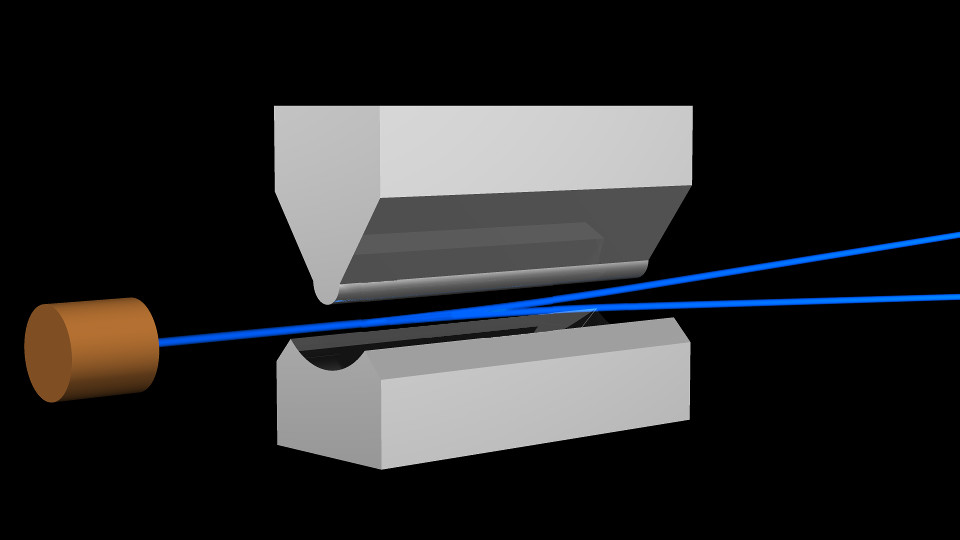
\includegraphics[width=\hsize]{graphics/sterngerlach.jpg}
\caption{Schematische Darstellung des Experimentes von Stern und
Gerlach: ein Strahl von Silber-Atomen wird durch ein inhomogenes
Magnetfeld in zwei Strahlen aufgeteilt.
\label{skript:sterngerlachimage}}
\end{figure}
Der Drehimpuls eines Elektrons in einem Atom "aussert sich ein einem
magnetischen Dipolmoment vom Betrag
\[
\frac{\hbar em}{m_e}.
\]
In einem inhomogenen Magnetfeld erf"ahrt ein Teilchen mit einem magnetischen
Moment eine von der Orientierung des magnetischen Dipolmomentes 
abh"angige Kraft.
Ein inhomogenes Magnetfeld sollte also
einen Strahl aus solchen Teilchen in mehrere Teilstrahlen
aufgeteilen, einen f"ur jeden m"oglichen Drehimpulszustand.

Dieses Experiment ist erstmals 1922 von Otto Stern und Walther Gerlach
mit einem Strahl von Silber-Atomen durchgef"uhrt
\index{Stern-Gerlach!Versuch von}
(Abbildung~\ref{skript:sterngerlachimage}).
Sie erwarteten die Aufspaltung in drei Teilstrahlen, die den
Werten $m=-1$, $m=0$ und $m=1$ entsprechen.
Beobachtet wurden aber nur zwei Strahlen, und vermuteten daher, dass
der Zustand $m=0$ fehle.

Erst 1925 wurde durch Goudsmith und Uhlenbeck postuliert, dass Elektronen
einen Eigendrehimpuls haben, der aber nur zwei Werte annehmen darf.
Die zugeh"origen Quantenzahlen mussten daher die Werte $l=\frac12$ und
$m=\frac12$ haben.
Es bestand aber immer noch die M"oglichkeit, dass die Aufspaltung
in nur zwei Teilstrahlen mit einem noch nicht verstandenen quantenmechanischen
Effekt in den doch recht komplizierten Silberatomen (Ordnungszahl 47)
erkl"art werden k"onnte.
Diese M"oglichkeit schlossen Experimente an Wasserstoffatomen
von Phipps und Taylor 1927 aus, die auch nur eine Aufspaltung
in zwei Strahlen zeigten.
Das Wasserstoffatom aus nur einem einzigen Eletron und einem Proton
ist sehr viel einfacher gebaut, es kann mit den Grundlagen
der Quantenmechanik bereits vollst"andig berechnet werden,
man darf annehmen, dass man das Wasserstoffatom versteht, und
schliessen, dass die Aufspaltung durch Spin verursacht wird.

%
% XXX man sollte von der zweiwertigkeit ausgehen, und am Schluss
% XXX erkennen, dass dieser Spin die gleichen Vertauschungsregeln
% XXX beinhaltet wie ein Drehimpuls
%
\section{Spin}
\rhead{Spin}
\begin{figure}
\centering
\includegraphics{graphics/spin-2.pdf}
\caption{Termschema f"ur die "Uberg"ange im Natrium-Atom, die zur gelben
Doppellinie (D-Linie) f"uhren.
\label{skript:natriumdlinie}}
\index{Natrium}
\end{figure}%
Die Experimente zeigen also , dass Elektronen sich verhalten, als k"onnten
sie trotz ihrer punktf"ormigen Geometrie rotieren.
Ein Elektron tr"agt also nicht nur seinen ganzzahligen Bahndrehimpuls,
der mit Hilfe der Drehimpulsoperatoren aus Kapitel~\ref{chapter:drehimpuls}
verstanden werden kann, sondern auch noch den halbzahligen Spin.

Bei "Uberg"angen zwischen Energiezust"anden muss auch der Gesamtdrehimpuls
aus Bahn\-dreh\-impuls und Spin erhalten bleiben.
Da Photonen ebenfalls einen Drehimpuls $\pm\hbar$ in Form zirkul"arer
Polarisierung 
haben, muss ein "Ubergang den Gesamtdrehimpuls des Atoms immer um genau
eine Drehimpulseinheit $\hbar$ "andern.
Der Elektronen-Spin stellt einen zus"atzlichen Freiheitsgrad dar, der die
Zahl der "Uberg"ange vermehrt.
Abbildung~\ref{skript:natriumdlinie} ist das (vereinfachte) Termschema f"ur 
Natrium, es zeigt zwei "Uberg"ange aus einem Zustand mit $l=1$ in einen
Zustand mit $l=0$ aus Zust"anden, die sich nur in der Orientierung
des Spins gegen"uber dem Bahndrehimpuls unterscheiden. 
Im Magnetfeld des Bahndrehimpuls entsteht eine Aufspaltung, die sich
in einer Aufspaltung der gelben Linie des Natriums "aussert.

%Es ist zwar nicht m"oglich, mit Hilfe der Drehimpulsoperatoren
%aus Kapitel~\ref{chapter:drehimpuls}
%dem Elektron einen Eigendrehimpuls zuzuteilen.
%Trotzdem kann man feststellen, dass im Elektron zus"atzlicher
%Drehimpuls stecken muss, denn gew"ohnlicher Drehimpuls kann verschwinden,
%da der Drehimpuls erhalten ist, muss er in das Elektron "ubergegangen
%sein.

Wir schliessen daraus, dass es einen Operator $\vec S$ gibt, der sich
genau so verh"alt wie ein Drehimpulsoperator, allerdings wirkt er nicht
auf die Ortskoordinaten.
Der Operator $\vec S$ heisst der Spin eines Elektrons.
\index{Elektronspin}%
Aus dem Stern-Gerlach-Experiment
weiss man ausserdem, dass Elektronen nur zwei verschiedene
Spinzust"ande haben k"onnen, was bedeutet, dass sich $\vec S$ wie ein
Drehimpulsoperator auf Zustandsvektoren mit $l=\frac12$ verh"alt.
Der Spin-Operator muss auf einen zweidimensionalen Hilbertraum
wirken, die Komponenten des Spin-Operators m"ussen also hermitesche
$2\times 2$-Matrizen sein, die die Vertauschungsrelationen eines
Drehimpulsoperators erf"ullen.

Die Matrizen $I$, $J$ und $K$ in (\ref{skript:komplex:definitionIJK}) haben
algebraische Eigenschaften, die nahe an dem sind, was wir suchen,
allerdings sind sie nicht hermitesch.
Multiplizieren wir sie mit $i$, erhalten wir die hermiteschen Matrizen
\begin{align}
\sigma_1
&=
\begin{pmatrix}
0&1\\1&0
\end{pmatrix}
&
\sigma_2
&=
\begin{pmatrix}
0&-i\\i&0
\end{pmatrix}
&
\sigma_3
&=
\begin{pmatrix}
1&0\\0&-1
\end{pmatrix}
\label{spin:paulimatrizen}
\end{align}
\index{Pauli-Matrizen}%
die auch {\em Pauli-Matrizen} genannt werden.
Diese Matrizen haben die folgenden Multiplikationseigenschaften:
\begin{align*}
%\sigma_1^2
%=
%\sigma_2^2
%=
%\sigma_3^2
%&=E,
%&
\sigma_1\sigma_2
&=
\begin{pmatrix} i&0\\0&-i \end{pmatrix} = i\sigma_3,
&
\sigma_2\sigma_3
&=
\begin{pmatrix} 0&i\\i&0 \end{pmatrix} = i\sigma_1,
&
\sigma_3\sigma_1
&=
\begin{pmatrix} 0&1\\-1&0 \end{pmatrix} = i\sigma_2,
\\
%&&
\sigma_2\sigma_1
&=
\begin{pmatrix} -i&0\\0&i \end{pmatrix} = -i\sigma_3,
&
\sigma_3\sigma_2
&=
\begin{pmatrix} 0&-i\\-i&0 \end{pmatrix} = -i\sigma_1,
&
\sigma_1\sigma_3
&=
\begin{pmatrix} 0&-1\\1&0 \end{pmatrix} = -i\sigma_2.
\end{align*}
\index{Pauli-Matrizen!Vertauschungsrelationen}%
Die Vertauschungsrelationen sind
\begin{align*}
[\sigma_1,\sigma_2]
&=
2i\sigma_3,
&
[\sigma_2,\sigma_3]
&=
2i\sigma_1,
&
[\sigma_3,\sigma_1]
&=
2i\sigma_2.
\end{align*}
Dies sind bis auf einen Faktor $\hbar/2$ die Vertauschungsrelationen,
die wir von einem Drehimpulsoperator erwarten,
daher k"onnen wir den Vektoroperator
\begin{equation}
\vec S=\frac{\hbar}2\vec\sigma
=
\frac{\hbar}2\begin{pmatrix}\sigma_1\\\sigma_2\\\sigma_3\end{pmatrix}
\label{spin:vektoroperator}
\end{equation}
als Spin-Operator verwenden.
\index{Spin-Operator}%
Der Betrag des Spin-Operators ist
\begin{align*}
\vec S^2
=
\frac{\hbar}{4}(\sigma_1^2+\sigma_2^2+\sigma_3^2)=\hbar^2\frac12\frac32E.
\end{align*}
Die Standardbasisvektoren sind Eigenvektoren sowohl von $\vec S^3$ wie
auch von $S_3$.
Wir bezeichnen sie daher auch $|\uparrow\rangle=e_1$ und
$|\downarrow\rangle=e_2$, es gilt:
\begin{align*}
\vec S^2\,|\uparrow\rangle&=\frac{3\hbar}4\,|\uparrow\rangle
&
\vec S^2\,|\downarrow\rangle&=\frac{3\hbar}4\,|\downarrow\rangle
\\
S_3\,|\uparrow\rangle&=\frac{\hbar}{2}\,|\uparrow\rangle
&
S_3\,|\downarrow\rangle&=-\frac{\hbar}{2}\,|\downarrow\rangle
\end{align*}

Die Auf- und Absteigeoperatoren f"ur den Spin sind
\index{Spin!Auf- und Absteigeoperatoren}%
\begin{align}
S_+
&=
S_1+iS_2
=
\frac{\hbar}2
(\sigma_1+i\sigma_2)
=
\frac{\hbar}2
\begin{pmatrix} 0&1+1\\1-1&0 \end{pmatrix}
=\hbar\begin{pmatrix}0&1\\0&0\end{pmatrix},
\\
S_-
&=
S_1-iS_2
=
\hbar\begin{pmatrix} 0&0\\1&0\end{pmatrix},
\\
S_+S_-+S_-S_+
&=
\hbar^2E,
\end{align}
genau wie f"ur den Operator $\vec L$.
Auf den Standardbasisvektoren wirken diese Operatoren wie
\begin{align*}
S_+\,|\uparrow\rangle&=0,
&
S_-\,|\uparrow\rangle&=\hbar\,|\downarrow\rangle,
\\
S_+\,|\downarrow\rangle&=\hbar\,|\uparrow\rangle,
&
S_-\,|\downarrow\rangle&=0.
\end{align*}
$S_+$ erh"oht also den Spin in $z$-Richtung, $S_-$ erniedrigt ihn.

\section{Spin im Magnetfeld}
\rhead{Spin im Magnetfeld}
Der Spin manifestiert sich durch seine Wechselwirkung mit einem
externen Magnetfeld.
Diese Wechselwirkung kann durch einen zus"atzlichen Term im
Hamilton-Operator modelliert werden.
Die Wechselwirkung eines magnetischen Dipolmoments mit einem
Magnetfeld $\vec B$ wird durch das Skalarprodukt gegeben,
der Hamilton-Operator, der sie ber"ucksichtigt, ist daher
\index{Spin!im Magnetfeld}%
% XXX Masseinheit: SI?
\[
H=H_0 + \frac{e}{m_e}\vec S\cdot\vec B.
\]
Darin ist $H_0$ der Hamilton-Operator ohne die Wechselwirkung 
zwischen Spin und Magnetfeld.

Wir k"onnen die St"orungstheorie verwenden, um den Einfluss eines
Magnetfeldes auf den Spin abzusch"atzen.
Da der ungest"orte Operator $H_0$ den Spin nicht enth"alt, gibt
es entartete Eigenzust"ande
$|\uparrow\rangle$ und $|\downarrow\rangle$
zu verschiedenen Spins, die aber sonst in allen Quantenzahlen
"ubereinstimmen.
Sie sind aber Eigenzust"ande des Spin-Magnetfeld-Operators
$\vec S\cdot \vec B$, so dass wir die St"orungstheorie anwenden
k"onnen.

In erster N"aherung sagt die St"orungstheorie, dass die Spin-Zust"ande
durch die St"orungstheorie nicht gemischt werden.
Nur die Energien werden sich "andern, und die "Anderung in 
Abh"angigkeit vom Magnetfeld k"onnen wir berechnen.

Wir nehmen an, dass das Magnetfeld nur eine $z$-Komponente $B_z$ hat,
dieses ist der St"orungsparameter.
Der Operator $H_1$ ist in dieser Basis durch die Matrix
\[
H_1=
\frac{\hbar e}{2m_e}
\begin{pmatrix}
1&0\\
0&-1
\end{pmatrix}
\]
gegeben.
Die St"orungstheorie liefert f"ur den linearen Koeffizienten von $B_z$
der Energie
\begin{align*}
E_\downarrow^{(1)}
&=
\langle \downarrow|\, H_1 \,|\downarrow\rangle
=\frac{\hbar e}{2m_e}
&
E_\uparrow^{(1)}
&=
\langle \uparrow|\, H_1 \,|\uparrow\rangle
=-\frac{\hbar e}{2m_e}
\end{align*}
Durch die St"orung werden die beiden Spin-Niveaus aufgespalten
in zwei Niveaus, deren Energie sich um
\[
\frac{\hbar e}{m_e}B_z
\]
unterscheidet.

\section{Spin und Statistik}
\rhead{Spin und Statistik}
\index{Spin!und Statistik}%
Die Theorie sagt aus, dass ein Teilchen nur einen totalen Spin haben kann,
der ein Vielfaches von $\frac12$ ist. Tats"achlich gibt es Teilchen
ganz ohne Spin, die $\pi$-Mesonen geh"oren dazu, aber auch das Higgs-Boson.
Elektronen, Protonen und Neutronen haben Spin $\frac12$. 
Atomkerne setzen sich aus vielen Protonen und Neutronen zusammen, ihr
Spin kann daher viel h"oher sein. Im Grundzustand haben jedoch auch
sie einen kleinen Spin.

\subsection{Austauschoperator\label{skript:austauschoperator}}
Ein einzelnes Teilchen hat in der Ortsdarstellung als Zustand
eine Wellenfunktion, die von den Ortskoordinaten und der Zeit abh"angt,
sie hat zwei Komponenten, eine f"ur jeden m"oglichen Spinzustand.
Wir k"onnten schreiben
\begin{equation}
|\psi\rangle
=
\begin{pmatrix}
\psi_\uparrow(x,y,z,t)\\
\psi_\downarrow(x,y,z,t)
\end{pmatrix}
\label{spin:vector}
\end{equation}
Statt die beiden m"oglichen Spinzust"ande durch einen Index zu unterscheiden,
k"onnten wir sie auch als Argumente der Wellenfunktion schreiben, also
als $\psi(x,y,z,t,s)$, wobei $s$ die Spinvariable ist. Der Zusammenhang
mit den Komponenten in (\ref{spin:vector}) ist
\[
\psi_\uparrow(x,y,z,t)
=
\psi(x,y,z,t,\uparrow)
\qquad\text{und}\qquad
\psi_\downarrow(x,y,z,t)
=
\psi(x,y,z,t,\downarrow).
\]
Wie sieht die Wellenfunktion eines Systems mit zwei Teilchen aus?
In die Wellenfunktion dieses Systems m"ussen die Koordinaten
$(x_1,y_1,z_1)$ und $(x_2,y_2,z_2)$ beider Teilchen eingehen, 
sowie die beiden Spins. Wir k"onnen die beiden Spins wieder als
Koordinaten einer Wellenfunktion
\[
|\psi_2\rangle
=
\psi_2(x_1,y_1,z_1,s_1,x_2,y_2,z_2,s_2,t)
\]
betrachten.
Elementarteilchen sind nicht unterscheidbar. Das bedeutet, dass sich
physikalisch nichts "andern darf, wenn wir die Koordinaten der beiden
Teilchen in $\psi_2$ vertauschen. Alle daraus berechneten physikalischen
Gr"ossen m"ussen gleich bleiben.

Wir k"onnen die Operation, die die Koordinaten vertauscht, also
Operator $A$ betrachten:
\index{Austauschoperator}%
\[
|\psi_2\rangle
=
\psi_2(x_1,y_1,z_1,s_1,x_2,y_2,z_2,s_2,t)
\mapsto
A|\psi_2\rangle
=
\psi_2(x_2,y_2,z_2,s_2,x_1,y_1,z_1,s_1,t)
\]
$A$ ist ein selbstadjungierter Operator.
Wendet man den Operator zweimal an, bleibt der Zustand unver"andert.
Der Operator $A$ erf"ullt also die Gleichung $A^2=\operatorname{id}$,
insbesondere kann $A$ nur Eigenwerte $\pm 1$ haben.
Ein Eigenzustand von $A$ erf"ullt also immer eine der beiden 
Gleichungen
\begin{align*}
A|\psi_2\rangle &= |\psi_2\rangle
\tag{symmetrisch}
\\
A|\psi_2\rangle &=-|\psi_2\rangle
\tag{antisymmetrisch}
\end{align*}
Wir k"onnen auch aus einem beliebigen Zustandsvektor $|\psi\rangle$
Eigenvektoren zu jedem $A$ bauen, indem wir
\begin{align*}
|\psi_\text{symmetrisch}\rangle
&=
\frac1{\sqrt{2}}(|\psi\rangle + A\,|\psi\rangle)
&
|\psi_\text{antisymmetrisch}\rangle
&=
\frac1{\sqrt{2}}(|\psi\rangle - A\,|\psi\rangle)
\end{align*}
bilden.

Wenn die beiden Teilchen nicht unterscheidbar sind, dann darf sich
die Energie nicht "andern, wenn die beiden Teilchen vertauscht
werden. Der Hamilton-Operator $H$ muss also mit $A$ vertauschen:
$[H,A]=0$. Wir k"onnen die Eigenzust"ande von $H$ also immer so
w"ahlen, dass sie auch Eigenzust"ande von $A$ sind.

Wenn $|\psi\rangle$ ein Eigenzustand von $H$ ist, dann muss auch
$|\psi_{\text{symmetrisch}}\rangle$ und
$|\psi_{\text{antisymmetrisch}}\rangle$ ein Eigenvektor sein.

\subsection{Pauli-Prinzip}
\index{Pauli-Prinzip}
Die Operator $H$ und $A$ erlaubten uns nicht zu entscheiden, welcher
der beiden Zust"ande $|\psi_{\text{symmetrisch}}\rangle$ und
$|\psi_{\text{antisymmetrisch}}\rangle$ in der Natur tats"achlich
vorkommt.
Experimentell hat man festgestellt, dass Teilchen mit halbzahligem
Spin, sogenannte Fermionen, nur mit einer antisymmetrischen
\index{Fermion}%
Wellenfunktion vorkommen k"onnen, w"ahrend Teilchen mit
ganzzahligem Spin, sogenannte Bosonen, nur mit einer symmetrischen
Wellenfunktion auftreten.
\index{Boson}

Wenn zwei Fermionen keine Wechselwirkung haben, dann k"onnen wir
aus zwei Wellenfunktionen
$\psi(x_1,y_1,z_1,s_1,t)$
und
$\psi(x_2,y_2,z_2,s_2,t)$
f"ur Fermionen eine antisymmetrische Wellenfunktion
\[
\psi_2(x_1,y_1,z_1,x_2,y_2,z_2,s_1,s_2,t)
=
\psi(x_1,y_1,z_1,s_1,t)
\psi(x_2,y_2,z_2,s_2,t).
\]
f"ur das Gesamtsystem bauen.
Wenn die beiden Fermionen den gleichen Spin haben, ist die
Funktion $\psi_2$ symmetrisch, kann also nicht die Wellenfunktion
eines Paares von Fermionen sein. 
Daraus leiten wir das Pauli-Prinzip ab:

\begin{satz}[Pauli-Prinzip]
Zwei Fermionen k"onnen nicht in einem Zustand sein, in dem alle
Quantenzahlen "ubereinstimmen.
\end{satz}
Zwei Fermionen m"ussen sich also in mindestens einer Quantenzahl
unterscheiden.
Zwei Elektronen k"onnen in einem Atom nur dann die gleichen
Energie- und Drehimpuls-Quantenzahlen haben, wenn sie sich im
Spin unterscheiden.

\subsection{Periodensystem}
\index{Periodensystem}%
Die Elektronen in einem Atom sind nicht voneinander unabh"angig,
jedes Elektron bewegt sich in einem Potential, welches vom Kern
und allen anderen Elektronen zusammen erzeugt wird.
In erster N"aherung k"onnen wir annehmen, dass alle Elektronen
das gleiche Potential sp"uren.
Selbst in dieser vereinfachten Situation schr"ankt das Pauli-Prinzip
die m"oglichen Elektronenzust"ande in einem Atom stark ein.
Keine zwei Elektronen k"onnen die gleichen Quantenzahlen f"ur
den Drehimpuls und den Spin haben.

Im Grundzustand werden in dieser N"aherung die Elektronen die Zust"ande
mit minimaler Energie ausw"ahlen.
In unserer Untersuchung des Wasserstoffatoms hat gezeigt, dass in
erster N"aherung die Energie nur von der Quantenzahlen $n$ abh"angt,
nicht von $l$, $m$ oder vom Spin, diese Energieniveaus sind entartet.

Die verschiedenen Drehimpulszust"ande werden durch die Spin-Bahn-Kopplung
aufgespalten (siehe Abbildung~\ref{skript:wasserstoffaufspaltung}).
Man kann sie sich als eine Wechselwirkung des vom Spin erzeugten
Magnetischen Momentes mit dem von der Bahnbewegung verursachten
Magnetfeld vorstellen.
Relativistische Effekte, die mit der Quantenelektrodynamik vollst"andig
verstanden werden k"onnen, sorgen daf"ur, dass in realen Atomen
die verschiedenen $m$-Werte zu leicht verschiedenen Energien f"uhren.
Die Wechselwirkung der verschiedenen Elektronenspins untereinander
spalten auch die letzten Niveaus noch auf.
Insgesamt k"onnen wir also davon ausgehen, dass alle Energieniveaus
verschieden sind.

Je gr"osser die Ladung des Kernes ist, desto mehr der m"oglichen
Elektronenzust"ande werden von Elektronen tats"achlich besetzt.
Die chemischen Eigenschaften eines Atoms h"angen davon ab, welche
Energie n"otig ist, ein Elektron zu entfernen oder hinzuzf"ugen.
Je nach den Quantenzahlen der Elektronen mit der gr"ossten Energie
werden sich die chemischen Eigenschaften "andern.
Man kann also erwarten, dass die Elemente "ahnliche Eigenschaften
zeigen, wenn ihre "aussersten Elektronen die gleichen $l$ und $m$
Quantenzahlen haben.

Das niedrigste Energieniveau ist $n=1$, in diesem Niveau gibt es
keine Zust"ande mit Drehimpuls $l\ne 0$. Es bleiben nur die
beiden Spin-Zust"ande, es gibt also nur zwei Atome, bei denen nur
die Zust"ande f"ur $n=1$ besetzt sind:
\begin{center}
\includegraphics{graphics/periodensystem-1.pdf}
\end{center}
Die Zust"ande der "aussersten Elektronen sind also solche mit
$l=0$, in dieser und den folgenden Tabelle sind sie rot
hinterlegt.
In Abschnitt~\ref{section:orbitale} haben wir diese Zust"ande unter
dem Namen s-Orbitale kennengelernt.

Wenn man mehr Elektronen hat, k"onnen auch die Zust"ande mit $n=2$ 
besetzt werden.
Hier gibt es insgesamt drei zus"atzliche Zust"ande mit Drehimpuls $l=1$,
die im Abschnitt~\ref{section:orbitale} p-Orbitale genannt wurden,
jeder mit zwei m"oglichen Spinzust"anden.
Die sechs Zust"ande f"ur $l=1$, die in der folgenden Tabelle 
gr"un hervorgehoben sind.
Es ist energetisch g"unstiger, als erstes einen der
Drehimpulszust"ande $l=0$ zu besetzen, und erst dann die Drehimpulszust"ande
mit $l=1$.
\begin{center}
\includegraphics{graphics/periodensystem-2.pdf}
\end{center}
Die Niveaus mit $l=2$
sind energetisch ung"unstiger
und kommen erst nach
den Niveaus f"ur $n=4$ und kleine Drehimpulse.

F"ur $n>3$ k"onnen die Niveaus mit $l=2$, die d-Orbitale, besetzt werden.
Zusammen mit
dem Spin gibt es zehn zus"atzliche Niveaus, die in der folgenden Tabelle
\footnote{Technetium (Tc) ist radioaktiv und daher in hellerer Farbe
\index{Technetium}%
dargestellt. Diese gilt auch f"ur das sp"ater dargestellte vollst"andige
Periodensystem.}
blau hervorgehoben sind.
\begin{center}
\includegraphics{graphics/periodensystem-3.pdf}
\end{center}

F"ur $n>5$ k"onnen schliesslich sogar die Niveaus $l=3$, die
f-Orbitale, besetzt werden.
Da es sieben Drehimpulszust"ande mit $l=3$ gibt, gibt es zusammen mit den
Spinzust"anden also vierzehn zus"atzliche Zust"ande, die in
der Tabelle gelb hervorgehoben sind
\begin{center}
\includegraphics[width=\hsize]{graphics/periodensystem-4.pdf}
\end{center}
Nat"urlich k"onnte man diese Tabelle noch viel weiter fortsetzen,
solange es aber keine so schweren Atomkerne gibt, sind solche Atome
nicht realisierbar.

